% !TEX TS-program = pdflatex
% !TEX encoding = UTF-8 Unicode

% This is a simple template for a LaTeX document using the ``article'' class.
% See ``book'', ``report'', ``letter'' for other types of document.

\documentclass[11pt]{article} % use larger type; default would be 10pt

\usepackage[utf8]{inputenc} % set input encoding (not needed with XeLaTeX)

%%% Examples of Article customizations
% These packages are optional, depending whether you want the features they provide.
% See the LaTeX Companion or other references for full information.

%%% PAGE DIMENSIONS
\usepackage{geometry} % to change the page dimensions
\geometry{a4paper} % or letterpaper (US) or a5paper or....
\geometry{margin=1in} % for example, change the margins to 2 inches all round
% \geometry{landscape} % set up the page for landscape
%   read geometry.pdf for detailed page layout information

\usepackage{graphicx} % support the \includegraphics command and options

% \usepackage[parfill]{parskip} % Activate to begin paragraphs with an empty line rather than an indent

%%% PACKAGES
\usepackage{booktabs} % for much better looking tables
\usepackage{array} % for better arrays (eg matrices) in maths
\usepackage{paralist} % very flexible & customisable lists (eg. enumerate/itemize, etc.)
\usepackage{verbatim} % adds environment for commenting out blocks of text & for better verbatim
\usepackage{subfig} % make it possible to include more than one captioned figure/table in a single float
% These packages are all incorporated in the memoir class to one degree or another...
\usepackage{enumitem}
\usepackage{amsmath}

% para los cuadritos en links
%\usepackage[linkbordercolor={0 0 1}, citebordercolor={0 1 0}, urlbordercolor={1 0 0}]{hyperref}
\usepackage[colorlinks=true, linkcolor=black, citecolor=green, urlcolor=red]{hyperref} % solo resalta
\usepackage[spanish]{babel}



%%% HEADERS & FOOTERS
\usepackage{fancyhdr} % This should be set AFTER setting up the page geometry
\pagestyle{fancy} % options: empty , plain , fancy
\renewcommand{\headrulewidth}{0pt} % customise the layout...
\lhead{}\chead{}\rhead{}
\lfoot{}\cfoot{\thepage}\rfoot{}

%%% SECTION TITLE APPEARANCE
\usepackage{sectsty}
\allsectionsfont{\sffamily\mdseries\upshape} % (See the fntguide.pdf for font help)
% (This matches ConTeXt defaults)

%%% ToC (table of contents) APPEARANCE
\usepackage[nottoc,notlof,notlot]{tocbibind} % Put the bibliography in the ToC
\usepackage[titles,subfigure]{tocloft} % Alter the style of the Table of Contents
\renewcommand{\cftsecfont}{\rmfamily\mdseries\upshape}
\renewcommand{\cftsecpagefont}{\rmfamily\mdseries\upshape} % No bold!

%%% END Article customizations

%%% The ``real'' document content comes below...

\title{Trabajo práctico 1\\ Redes Neuronales y Aprendizaje Profundo}
\author{Ignacio Ezequiel Cavicchioli\\Padrón 109428\\icavicchioli@fi.uba.ar}
\date{10/9/2025} % Activate to display a given date or no date (if empty),
         % otherwise the current date is printed



\begin{document}
\maketitle

\tableofcontents



\section{Introducción}

Este documento presenta el desarrollo de las consignas del trabajo práctico N°2 de la materia de \textbf{Redes Neuronales y Aprendizaje Profundo}.  El código correspondiente fue realizado en  \textit{Jupyter notebooks}, \textit{Python}, adjuntados a la entrega en formato PDF. Toda imagen o implementación requeridas para el análisis se explicitarán en el presente archivo, por lo que la lectura del código en sí queda a discreción del lector. La teoría relevante será presentada y discutida en la sección pertinente.


\newpage

\section{Ejercicio 1}

\subsection{Consignas}

Implemente un perceptrón simple que aprenda la función lógica AND y la función lógica OR, de 2 y de 4 entradas. Muestre la evolución del error durante el entrenamiento. Para el caso de 2 dimensiones, grafique la recta discriminadora y todos los vectores de entrada de la red.

\subsection{Desarrollo}

Lo primero que se hizo fue generar el dataset para entrenar los perceptrones, que no es más que la tabla de verdad de la función lógica que se quiere aprender.

Las figuras \ref{fig:and2err}, \ref{fig:and4},\ref{fig:or2err},\ref{fig:or4} muestran el error en función de la iteración (de entrenamiento) para los perceptrones que emulan las funciones AND y OR de 2 y 4 entradas. Como se discutió en la teórica, el perceptrón es capaz de aprender estas funciones lógicas simples, por lo que el error final del entrenamiento es cero.

La figura \ref{fig:orfront} muestra la frontera de decisión del perceptrón que aprendió la función OR, y la \ref{fig:frontAND} muestra la frontera para la compuerta AND. Los puntos del mismo color son de la misma clase (0 o 1), y son adecuadamente segregados por la frontera. Contrario a SVM, el perceptrón simple no tiene la distancia desde la frontera hasta las muestras en su función de costo, por lo que la recta que separa las clases no es única.

Para encontrar la fórmula de la recta que hace de frontera de decisión se puede partir de la expresión de la sumatoria de los $X$ con sus respectivos pesos y el bias, y suponer que $Y=0$, lo que significa que estás parado sobre la frontera, tu muestra no es ni de una clase ni de la otra.

$$
X1 \cdot w1 + X2 \cdot w2 + b = 0
$$

Y si suponemos que $X1$ es nuestra abscisa que vamos a barrer y $X2$ es la ordenada, la recta toma la forma de:

$$
X2 = \frac{w1 \cdot X1 + b}{-w2}
$$

Y entonces $m=-w1/w2 $ y b = $-b/w2$

\begin{figure}[h!]
	\centering
	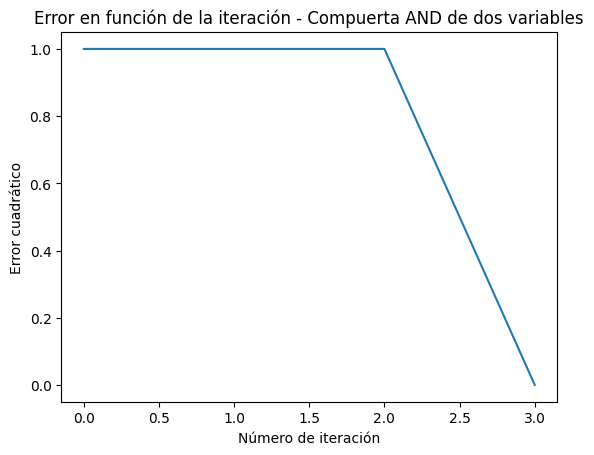
\includegraphics[width=0.7\linewidth]{../imgs/ej1/AND2err}
	\caption[]{Error de entrenamiento en el tiempo para compuerta AND de 2 entradas}
	\label{fig:and2err}
\end{figure}


\begin{figure}[h!]
	\centering
	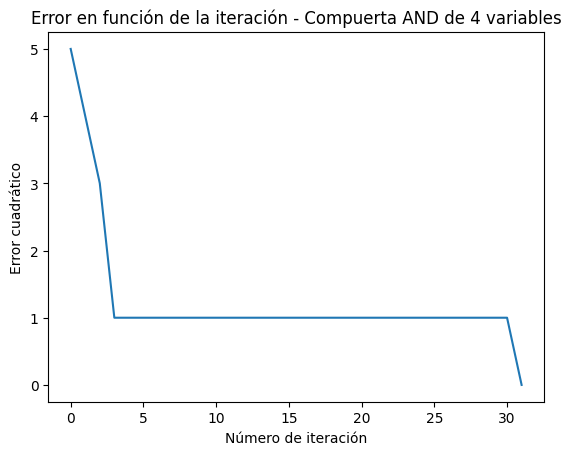
\includegraphics[width=0.7\linewidth]{../imgs/ej1/AND4}
	\caption[]{Error de entrenamiento en el tiempo para compuerta AND de 4 entradas}
	\label{fig:and4}
\end{figure}



\begin{figure}[h!]
	\centering
	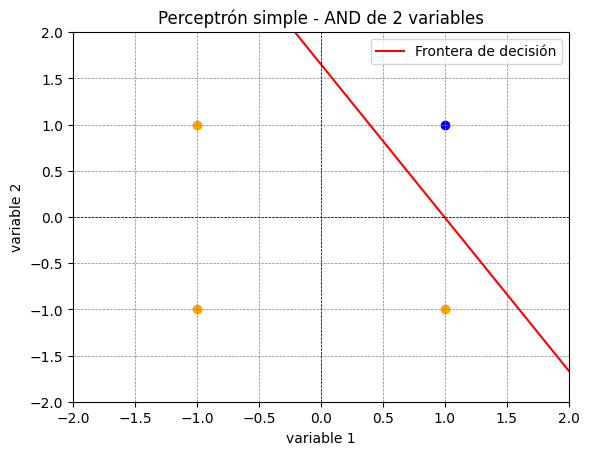
\includegraphics[width=0.7\linewidth]{../imgs/ej1/ANDFRONT}
	\caption[]{Frontera encontrada para compuerta AND de 2 entradas}
	\label{fig:frontAND}
\end{figure}

\begin{figure}[h!]
	\centering
	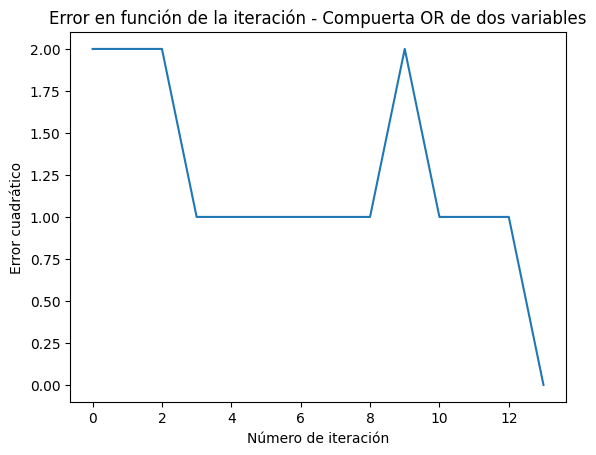
\includegraphics[width=0.7\linewidth]{../imgs/ej1/OR2err}
	\caption[]{Error de entrenamiento en el tiempo para compuerta OR de 2 entradas}
	\label{fig:or2err}
\end{figure}

\begin{figure}[h!]
	\centering
	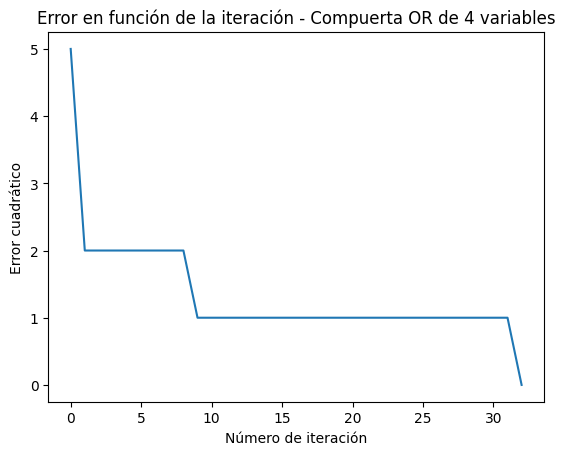
\includegraphics[width=0.7\linewidth]{../imgs/ej1/OR4}
	\caption[]{Error de entrenamiento en el tiempo para compuerta OR de 4 entradas}
	\label{fig:or4}
\end{figure}

\begin{figure}[h!]
	\centering
	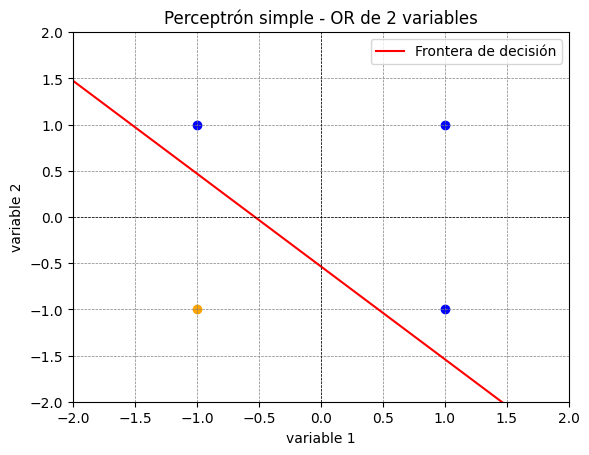
\includegraphics[width=0.7\linewidth]{../imgs/ej1/ORFRONT}
	\caption[]{Frontera encontrada para compuerta OR de 2 entradas}
	\label{fig:orfront}
\end{figure}


\subsection{Análisis}

Los perceptrones lograron aprender sus funciones lógicas designadas sin error en una cantidad finita de iteraciones del algoritmo.

El ejercicio demuestra la capacidad del perceptrón de aprender, además de familiarizarnos con un algoritmo de gradiente descendiente, por el cual los pesos se actualizan en la dirección que minimiza el error.

Todo esto es fundamental para las consignas siguientes.


\clearpage

\section{Ejercicio 2}

\subsection{Consignas}

Determine numéricamente cómo varía la capacidad del perceptrón simple en función del número de patrones enseñados.


\subsection{Desarrollo}

La capacidad de un perceptron está definida en la p.111 del libro ``Introduction to the theory of neural computation''. El experimento se debe hacer para para una cantidad particular de unidades de entrada, que sería la dimensión de nuestro espacio de features. A medida que este número N aumenta ($N \to \inf$), se demuestra que la capacidad de almacenamiento máxima del perceptron converge a $p_{max} = 2N$, con $p$ la cantidad de patrones.

La idea es tomar un perceptron de cierto tamaño y alimentarlo con cada vez más patrones, registrando los resultados.
En el ejercicio, la capacidad se ensayó de la siguiente forma:

los resultados para $N=30$ se pueden ver en la figura \ref{fig:capacidad}.

\begin{figure}[h!]
	\centering
	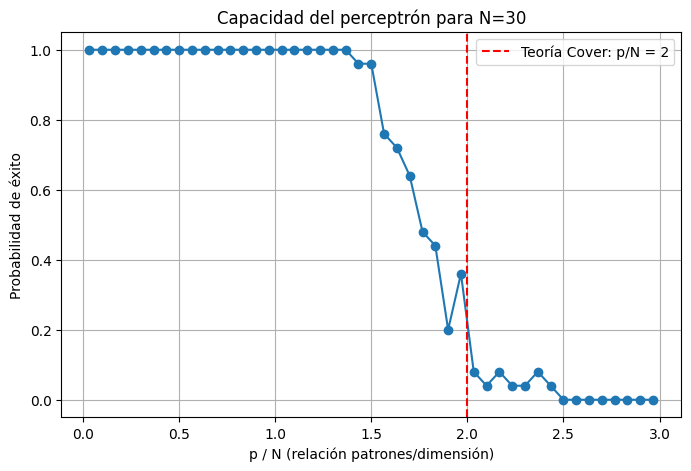
\includegraphics[width=0.7\linewidth]{../imgs/ej2/capacidad}
	\caption[]{Ensayo de capacidad $N=30$}
	\label{fig:capacidad}
\end{figure}


\subsection{Análisis}

\clearpage

\section{Ejercicio 3}

\subsection{Consignas}

Implemente un perceptrón multicapa que aprenda la función lógica XOR de 2 y de 4 entradas (utilizando el algoritmo Backpropagation y actualizando en batch). Muestre cómo evoluciona el error durante el entrenamiento.

\subsection{Desarrollo}
\begin{figure}
	\centering
	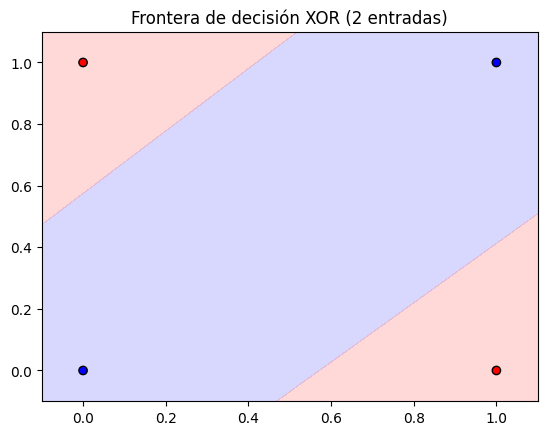
\includegraphics[width=0.7\linewidth]{imgs/ej3_frontera_xor}
	\caption{}
	\label{fig:ej3fronteraxor}
\end{figure}


\begin{figure}
	\centering
	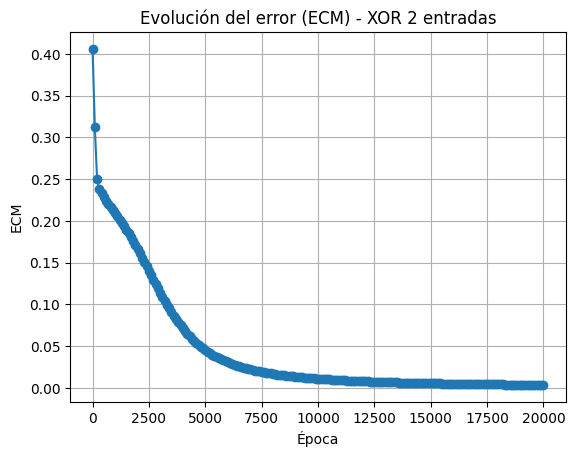
\includegraphics[width=0.7\linewidth]{imgs/ej3__error_xor2}
	\caption{}
	\label{fig:ej3errorxor2}
\end{figure}

\begin{figure}
	\centering
	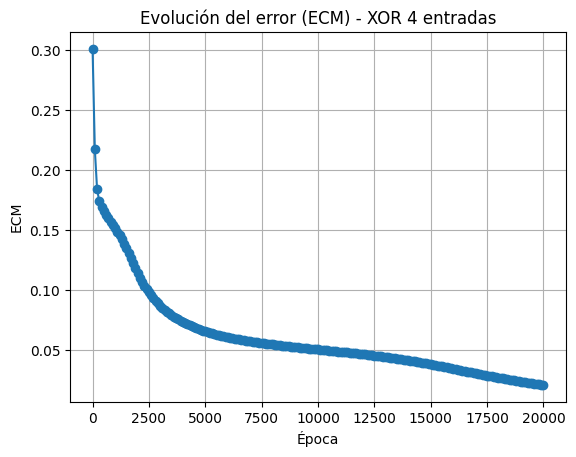
\includegraphics[width=0.7\linewidth]{imgs/ej3__error_xor4}
	\caption{}
	\label{fig:ej3errorxor4}
\end{figure}


\subsection{Análisis}

\clearpage

\section{Ejercicio 4}

\subsection{Consignas}

a - Implemente una red con aprendizaje Backpropagation que aprenda la siguiente función:
$$
f (x , y , z)= \sin(x)+\cos(y)+z
$$

donde: $x$ e $y$ $\in [0,2 \pi]$ y $z \in [-1,1]$.

Para ello construya un conjunto de datos de entrenamiento y un conjunto de evaluación. Muestre la evolución del error de entrenamiento y de evaluación en función de las épocas de entrenamiento.

b - Estudie la evolución de los errores durante el entrenamiento de una red con una capa oculta de 30 neuronas cuando el conjunto de entrenamiento contiene 40 muestras. ¿Que ocurre si el minibatch tiene tamaño 40? ¿Y si tiene tamaño 1?

\subsection{Desarrollo}

\subsection{Análisis}




\clearpage

\section{Ejercicio 5}

\subsection{Consignas}

Siguiendo el trabajo de Hinton y Salakhutdinov (2006), entrene una máquina restringida de Boltzmann con imágenes de la base de datos MNIST. Muestre el error de reconstrucción durante el entrenamiento, y ejemplos de cada uno de los dígitos reconstruidos.
\subsection{Desarrollo}

\subsection{Análisis}

\clearpage

\section{Ejercicio 6}

\subsection{Consignas}

Entrene una red convolucional para clasificar las imágenes de la base de datos MNIST.
¿Cuál es la red convolucional más pequeña que puede conseguir con una exactitud de al menos 90\% en el conjunto de evaluación? ¿Cuál es el perceptrón multicapa más pequeño que puede conseguir con la misma exactitud?

\subsection{Desarrollo}

\subsection{Análisis}


\clearpage

\section{Ejercicio 7}

\subsection{Consignas}

Entrene un autoencoder para obtener una representación de baja dimensionalidad de las imágenes de MNIST. Use dichas representaciones para entrenar un perceptrón multicapa como clasificador. ¿Cuál es el tiempo de entrenamiento y la exactitud del clasificador obtenido cuando parte de la representación del autoencoder, en comparación con lo obtenido usando las imágenes originales?

\subsection{Desarrollo}

\begin{figure}[h!]
	\centering
	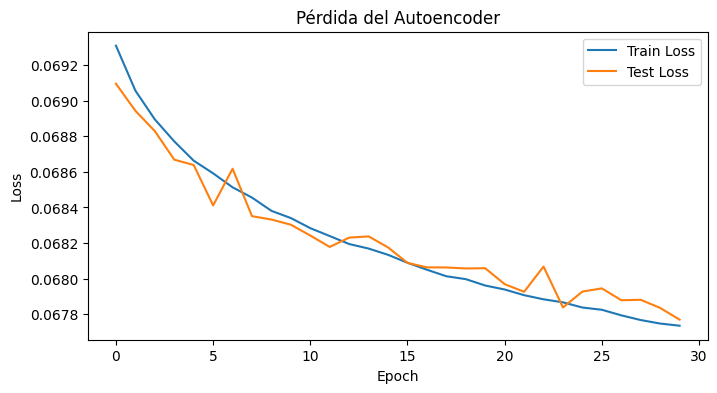
\includegraphics[width=0.7\linewidth]{imgs/ej7_loss}
	\caption{}
	\label{fig:ej7loss}
\end{figure}

\begin{figure}[h!]
	\centering
	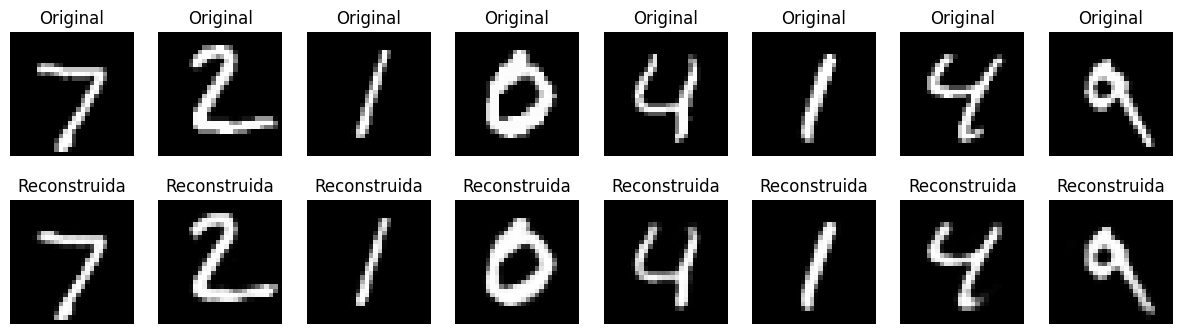
\includegraphics[width=0.7\linewidth]{imgs/ej7_reconstr_digitos}
	\caption{}
	\label{fig:ej7reconstrdigitos}
\end{figure}

entrenamiento final:
Epoch 1/30 | Loss=0.6624 | Acc=81.28%
Epoch 2/30 | Loss=0.3537 | Acc=89.86%
Epoch 3/30 | Loss=0.3200 | Acc=90.68%
Epoch 4/30 | Loss=0.3073 | Acc=90.92%
Epoch 5/30 | Loss=0.2996 | Acc=91.19%
Epoch 6/30 | Loss=0.2962 | Acc=91.22%
Epoch 7/30 | Loss=0.2921 | Acc=91.29%
Epoch 8/30 | Loss=0.2884 | Acc=91.44%
Epoch 9/30 | Loss=0.2884 | Acc=91.51%
Epoch 10/30 | Loss=0.2855 | Acc=91.53%
Epoch 11/30 | Loss=0.2832 | Acc=91.62%
Epoch 12/30 | Loss=0.2837 | Acc=91.56%
Epoch 13/30 | Loss=0.2823 | Acc=91.63%
Epoch 14/30 | Loss=0.2813 | Acc=91.79%
Epoch 15/30 | Loss=0.2810 | Acc=91.69%
Epoch 16/30 | Loss=0.2799 | Acc=91.83%
Epoch 17/30 | Loss=0.2785 | Acc=91.79%
Epoch 18/30 | Loss=0.2773 | Acc=91.82%
Epoch 19/30 | Loss=0.2772 | Acc=91.85%
Epoch 20/30 | Loss=0.2775 | Acc=91.76%
Epoch 21/30 | Loss=0.2751 | Acc=91.91%
Epoch 22/30 | Loss=0.2738 | Acc=91.90%
Epoch 23/30 | Loss=0.2745 | Acc=91.89%
Epoch 24/30 | Loss=0.2738 | Acc=91.94%
Epoch 25/30 | Loss=0.2735 | Acc=91.97%
...
Epoch 28/30 | Loss=0.2736 | Acc=91.98%
Epoch 29/30 | Loss=0.2726 | Acc=91.98%
Epoch 30/30 | Loss=0.2720 | Acc=92.05%
Test Accuracy: 92.33%




\subsection{Análisis}

\clearpage


\section{Conclusiones}

\end{document}
